\documentclass[a4paper,12pt,oneside]{book}

\usepackage{localfmt}
\usepackage{localshortcuts}

\def\withsolution{1}

\def\withgrading{1}

\begin{document}

\titlePageB{Интеллектуальные робототехнические системы}

\setcounter{tocdepth}{1}

\tableofcontents

\chapter{Введение}

Олимпиада Национальной технологической инициативы  (далее – Олимпиада \linebreak НТИ)\footnote{Национальная технологическая инициатива (НТИ) — это программа мер, нацеленная на формирование принципиально новых рынков и создание условий для глобального технологического лидерства России к 2035 году. Задача по созданию НТИ поставлена Президентом Российской Федерации 4 декабря 2014 года в Послании к Федеральному собранию.} – это командная инженерная олимпиада школьников, завершающаяся разработкой действующего устройства, системы устройств или компьютерной программы. Олимпиада является проектом Агентства стратегических инициатив, элементом дорожной карты НТИ «Кружковое движение» и ключевым механизмом вовлечения инженерно – ориентированных школьников в образовательные программы высшего образования, ориентированные на рынки НТИ. Оператором Олимпиады НТИ  является некоммерческая организация – Ассоциация участников технологических кружков. Профили Олимпиады НТИ выбраны на основе приоритетов Национальной технологической инициативы: «Автономные транспортные системы», «Большие данные и машинное обучение», «Системы связи и дистанционного зондирования Земли», «Интеллектуальные энергетические системы», «Нейротехнологии», «Инженерные биологические системы: агробиотехнологии и геномное редактирование», «Интеллектуальные робототехнические системы», «Беспилотные авиационные системы», «Композитные технологии», «Когнитивные технологии», «Аэрокосмические системы», «Наносистемы и наноинженерия», «Технологии беспроводной связи», «Умный город», «Передовые производственные технологии», «Виртуальная и дополненная реальность», «Анализ космических снимков и геопространственных данных», «Водные робототехнические системы» и «Программная инженерия финансовых технологий».

Цель Олимпиады НТИ: поддержка школьников в стремлении решать технологические вызовы XXI века (что подразумевает включение их в решение технологических задач переднего края и, одновременно, повышение социальной значимости такой работы старшеклассников через льготы к поступлению). Эта цель лежит в рамках большей цели Кружкового движения: формирование и подготовка команд, способных запускать глобальные технологические проекты, менять мир, создавая новые общественные практики. Именно участники этих команд должны будут через 10-15 лет «перезапустить» НТИ: создать собственные рынки и глобальные прорывные компании.  Важной особенностью олимпиады является то, что в части отборочного и в заключительном этапах участники выполняют задания в командах по 2-4 человека. Умение работать в команде - важный навык человека 21 века. Команды формируются на основе компетентностного принципа, различные компетенции участников в одной команде позволяют найти оригинальное нестандартное решение задачи.  В командах участники планируют свою работу, обсуждают, ищут совместно решения, распределяют роли - часто один участник выполняет несколько ролей. Комплексные инженерные задачи, которые решают участники, не под силу решить отдельно взятому школьнику. Задачи разработаны таким образом, что декомпозируются на несколько подзадач, за решение, которых берутся участники согласно своей роли в команде. Каждый участник несет ответственность за результат работы команды. Поэтому, при подведении итогов олимпиады определяются не только победители в личном зачете, но и команда-победитель. 

Целевыми победителями Олимпиады НТИ являются школьники, способные реализовывать сложные технические проекты в прорывных областях. Олимпиада должна выделять команды участников с особыми характеристиками мышления, коммуникации и действия, необходимыми для решения задач НТИ. Победители и призеры Олимпиады НТИ должны показывать высокие результаты в области применения предметных знаний в практической работе. Одновременно с этим, система подготовки Олимпиады НТИ должна предоставлять участникам инструменты для подготовки и получения недостающих знаний и практических навыков.

\section*{Первый год проведения олимпиады}

Олимпиада НТИ была впервые проведена в 2015/2016 учебном году. В отборочных этапах олимпиады приняли участие несколько тысяч школьников, около ста из них были приглашены к участию в заключительном этапе по профилям «Большие данные и машинное обучение», «Системы связи и дистанционного зондирования Земли», «Интеллектуальные энергетические системы», «Автономные транспортные системы». Заключительный этап Олимпиады и торжественные мероприятия проводились в ВДЦ «Орленок». 

В 2015/2016 учебном году победители и призеры олимпиады могли воспользоваться возможностью добавить дополнительные 10 баллов к сумме баллов за вступительные экзамены, в случае если они поступали в вузы-организаторы Олимпиады НТИ. 

\section*{Второй год проведения олимпиады}

В 2016/2017 учебном году Олимпиада проводилась во второй раз по 12 профилям, количество зарегистрированных для участия школьников увеличилось более чем в три раза и достигло 12 тыс., в отборочных этапах приняли активное участие 4 тыс. школьников, на заключительный этап прибыло 306 участников.  

Заключительный этап Олимпиады и торжественные мероприятия проводились на площадке Образовательного центра «Сириус», в лабораториях и помещениях Парка Наук и Искусств. Вечером проходили лекции и неформальные встречи с представителями технологических компаний. 

В 2016/2017 учебном году четыре профиля Олимпиады НТИ («Автономные транспортные системы», «Большие данные и машинное обучение», «Системы связи и дистанционного зондирования Земли», «Интеллектуальные энергетические системы») входили в Перечень олимпиад школьников, таким  образом победители и призеры смогли воспользоваться льготами при поступлении в вузы России (в зависимости от правил приема конкретного вуза). Победители и призеры новых профилей также могли воспользоваться бонусами при поступлении в вузы, которые имеют статус «организатор Олимпиады НТИ».

\section*{Третий год проведения олимпиады}

В отборе на Олимпиаду 2017/2018 учебного года приняло участие более 20 тыс. школьников, подавших более 50 тыс. заявок на различные профили, число которых увеличилось до 17. В финал вышли 578 участников Олимпиады из 51 региона РФ:

\putImgWOCaption{16cm}{history/info/map}

Финал стал распределенным и проходил с февраля по апрель 2018 года: Олимпиаду приняли Образовательный центр «Сириус», МАИ, МИФИ, ТПУ, Университет Иннополис, СПбПУ, ДВФУ, УрФУ. В 2017/2018 учебном году девять из 14 профилей Олимпиады НТИ включены в Перечень олимпиад школьников (приказ Минобрнауки России от 30.08.2017 № 866) и дают льготы при поступлении в вузы.

Важная составляющая подготовки участников к финалу Олимпиады –  открытые для всех желающих хакатоны, вебинары и мастер-классы. Программы этих мероприятий разработаны педагогами профилей Олимпиады НТИ специально для регионов так, чтобы их можно было провести на минимальном количестве оборудования. Сеть региональных партнеров Олимпиады со статусом Методическая площадка или Площадка подготовки растет с каждым годом, и в 2018 году, на третий год проведения Олимпиады, их количество достигло 110, всего проведенных мероприятий по подготовке  (соревнований, хакатонов, сборов) –  более 50. Информация о партнерских площадках размещена в специальном разделе официального сайта олимпиады: \url{http://nti-contest.ru/places_to_prepare/}.

\section*{Четвертый год проведения олимпиады}

В отборе на Олимпиаду 2018/2019 учебного года приняло участие более 36 тыс. школьников, подавших более 70 тыс. заявок на различные профили, число которых увеличилось до 19. В финал вышли 1053 участника Олимпиады из 60 регионов РФ.

Финал стал распределенным и проходил с марта по апрель 2019 года: Олимпиаду приняли МФТИ, МАИ, МИФИ, ТПУ, Университет Иннополис, СПбПУ, ДВФУ, НГУ, НовГУ, Московский Политех, ИГУ, ИРНИТУ и ряд других площадок. В 2018/2019 учебном году 13 из 19 профилей Олимпиады НТИ включены в Перечень олимпиад школьников (приказ №32н от 28 августа 2018 года Министерства науки и высшего образования Российской Федерации) и дают льготы при поступлении в вузы.

В олимпиаде в 2018/2019 учебном году впервые были проведены синхронные по времени распределенные финалы на площадках в разных городах в рамках одного профиля: Нейротехнологии (ДВФУ, НГУ, МФТИ, НовГУ), ИЭС (ИГУ, МИФИ), Нанотехнологии (Школа Летово, НГУ), АТС (Московский политех, НовГУ). Участники распределенных финалов имели одинаковые задания, критерии оценивания и единый рейтинг участников.

\section*{График проведения заключительных этапов\\Олимпиады НТИ 2018/2019 гг.}

\begin{center}
    \small
    \begin{longtable}{|p{7.5cm}|p{2.5cm}|p{5cm}|}
        \hline
        \textbf{Площадка проведения} & \textbf{Даты проведения} & \textbf{Перечень профилей Олимпиады НТИ} \\
        \hline
        \textbf{Университет Иннополис}
        
        (г. Иннополис) & 3-11 марта 2019 г. & Интеллектуальные робототехнические системы\\
        \hline
        \textbf{Университет Иннополис}
        
        (г. Иннополис) & 6-11 марта 2019 г. & Программная инженерия финансовых технологий\\
        \hline
        \textbf{Школа Летово}

        (г. Москва)

        \textbf{Новосибирский государственный университет}

        (г. Новосибирск) & 11-16 марта 2019 г. & Наносистемы и наноинженерия \\
        \hline
        \textbf{Московский политехнический университет} 

        (г. Москва) & 11-16 марта 2019 г. & Инженерные биологические системы: Агробиотехнологии \\
        \hline
        \textbf{Московский авиационный институт}

        (г. Москва) & 11-16 марта 2019 г. & Беспилотные авиационные системы \\
        \hline
        \textbf{Томский политехнический университет} 

        (г. Томск) & 12-17 марта 2019 г. & Умный город \\
        \hline
        \textbf{Иркутский национальный исследовательский технический университет}

        (г. Иркутск) & 13-19 марта 2019 г. & Технологии беспроводной связи\\
        \hline
        \textbf{Иркутский государственный университет} 

        (г. Иркутск)

        \textbf{Национальный исследовательский ядерный университет «МИФИ»}
        
        (г. Москва) & 13-19 марта 2019 г. & Интеллектуальные энергетические системы \\
        \hline
        \textbf{Иркутский государственный университет} 

        (г. Иркутск) & 13-19 марта 2019 г. & Технологии виртуальной и дополненной реальности: Дополненная реальность\\
        \hline
        \textbf{Дальневосточный федеральный университет}

        (г. Владивосток) & 18-23 марта 2019 г. & Виртуальная и дополненная реальность: Виртуальная реальность \\
        \hline
        \textbf{Дальневосточный федеральный университет} 

        (г. Владивосток) & 18-23 марта 2019 г. & Водные робототехнические системы \\
        \hline
        \textbf{Московский физико-технический институт}

        (г. Москва)

        \textbf{Новосибирский государственный университет}

        (г. Новосибирск) 

        \textbf{Новгородский государственный университет имения Ярослава Мудрого}

        (г. Великий Новгород)

        \textbf{Дальневосточный федеральный университет}

        (г. Владивосток) & 18-23 марта 2019 г. & Нейротехнологии \\
        \hline 
        \textbf{Московский физико-технический институт}

        (г. Москва),

        \textbf{Новосибирский государственный университет}

        (г. Новосибирск) & 18-23 марта 2019 г. & Инженерные биологические системы: Геномное редактирование \\
        \hline
        \textbf{Московский физико-технический институт}

        (г. Москва) & 18-23 марта 2019 г. & Большие данные и машинное обучение \\
        \hline
        \textbf{АО «ИПК Машприбор» ГК Роскосмос} 

        (г. Королев)

        \textbf{Детский технопарк «Кванториум»}

        (г. Королев) & 26-31 марта 2019 г. & Системы связи и дистанционного зондирования Земли \\
        \hline
        \textbf{АО «ИПК Машприбор» ГК Роскосмос}

        (г. Королев)

        \textbf{Детский технопарк «Кванториум»}

        (г. Королев) & 26-31 марта 2019 г. & Аэрокосмические технологии \\
        \hline
        \textbf{АО «ИПК Машприбор» ГК Роскосмос}

        (г. Королев)

        \textbf{Детский технопарк «Кванториум»}

        (г. Королев) & 26-31 марта 2019 г. & Анализ космических снимков и пространственных геоданных Земли \\
        \hline
        \textbf{Санкт-Петербургский университет Петра Великого,}

        \textbf{Академия цифровых технологий}

        (г. Санкт-Петербург) & 01-06 апреля 2019 г.	& Передовые производственные технологии \\
        \hline
        \textbf{Московский государственный психолого-педагогический университет}
        
        (г. Москва) & 02-06 апреля 2019 г. & Когнитивные технологии \\
        \hline
        \textbf{Московский государственный технический университет им. Н.Э. Баумана}

        (г. Москва) & 07-12 апреля 2019 г. & Композитные технологии \\
        \hline
        \textbf{Московский политехнический университет}
        (г. Москва)

        \textbf{Новгородский государственный университет имения Ярослава Мудрого}

        (г. Великий Новгород) & 08-14 апреля 2019 г. & Автономные транспортные системы\\
        \hline        
    \end{longtable}
\end{center}

\section*{Организаторы и партнеры Олимпиады НТИ}

Оргкомитет олимпиады представлен ректорами крупнейших политехнических и инженерных вузов России, руководителями технологических компаний и представителями государственных органов.

\textbf{Вузы-соучредители олимпиады:}
\begin{itemize}
    \item ФГБОУ ВО «Московский политехнический университет»;
    \item ФГАОУ ВО «Санкт-Петербургский политехнический университет Петра Великого»;
    \item ФГАОУ ВО «Национальный исследовательский Томский политехнический университет»;
    \item ФГАОУ ВО «Дальневосточный федеральный университет».
\end{itemize}

\textbf{Технологические партнеры}

Олимпиада НТИ проводится при поддержке технологических партнеров, количество которых увеличилось, по сравнению с прошлым годом,  среди них: РВК (Российская венчурная компания) и АСИ (Агентство стратегических инициатив по продвижению новых проектов)  –  в роли со-организаторов и генеральных партнеров выступают: Аэрофлот, ПАО «Сухой», ОАК, Роскосмос, ФИОП Роснано, МТС, Газпром нефть, Фонд новых форм развития образования, сеть детских технопарков «Кванториум», Спутникс, Полюс-НТ, BiTronicsLab, КРОК,  Инфосистемы Джет, Лоретт, Коптер Экспресс, АсРоботикс, Образование будущего и др. Полный список организаторов и партнеров олимпиады размещен в соответствующем разделе на официальном сайте: \url{http://nti-contest.ru/about/}.

\textbf{Вузы-организаторы профилей Олимпиады НТИ:}
\begin{itemize}
    \item АНО ВО «Университет Иннополис»; 
    \item ФГАОУ ВО «Национальный исследовательский ядерный университет «МИФИ»;
    \item ФГАОУ ВО «Московский физико-технический институт (государственный университет)»;
    \item ФГБОУ ВО «Московский авиационный институт (национальный исследовательский университет)»;
    \item ФГБОУ ВО «Сибирский государственный университет науки и технологий имени академика М.Ф. Решетнева»;
    \item ФГАОУ ВО «Новосибирский национальный исследовательский государственный университет»;
    \item АНО ВО «Сколковский институт науки и технологий»;
    \item ФГБОУ ВО «Московский государственный психолого-педагогический университет»;
    \item ФГБОУ ВО «Московский государственный технический университет имени Н.Э. Баумана (национальный исследовательский университет)»;
    \item ФГБОУ ВО «Новгородский государственный университет имени Ярослава Мудрого»;
    \item ФГБОУ ВО «Иркутский государственный университет»;
    \item ФГБОУ ВО «Новосибирский государственный технический университет»;
    \item ФГАОУ ВО «Национальный исследовательский Нижегородский государственный университет им. Н.И. Лобачевского»;
    \item ФГБОУ ВО «Московский технический университет связи и информатики».
\end{itemize}

К работе методической комиссии был привлечен профессорско-преподавательский состав вузов-организаторов и представители реального сектора экономики. Объективную оценку работы осуществляет жюри, представленное основателями технологических компаний, а также представителями вузов-организаторов.  

Вузы-организаторы, входящие в Оргкомитет Олимпиады НТИ, ведут непрерывную работу с талантливыми школьниками.

\textbf{Университет Иннополис:}

Университет Иннополис – интеллектуальное ядро нового города и российский университет, который специализируется на образовании и научных исследованиях в области современных информационных технологий. Основная цель создания университета – подготовка высококвалифицированных кадров по ИТ -специальностям. В рамках работы над этой целью в университете организовано подразделение по подготовке школьников. Основное направление работы подразделения – это выявление и развития талантливых школьников, а также развитие IT компетенций в регионе и стране.

В течение года университет проводит большое количество образовательных мероприятий и интеллектуальных конкурсов по различным направлениям. 

Работа по выявлению и развитию талантов школьников проходит по шести направлениям:\
\begin{itemize}
    \item Регулярные занятия
    \item Региональные образовательные смены
    \item Федеральные образовательные смены
    \item Инженерные, научно-технические конкурсы, соревнования и олимпиады
    \item Учебно-тренировочные сборы для финалистов, представителей республики и страны
    \item Курсы повышения квалификации для педагогов
\end{itemize}

Регулярные занятия проводятся для учащихся 4 – 11 классов на площадках школ города Казань, города Иннополис и Университета Иннополис по направлениям «программирование», «олимпиадное программирование», «математика», «олимпиадная математика», «олимпиадная робототехника», «прототипирование и 3D моделирование» и «компьютерное зрение». 

Региональные образовательные смены проводятся в каникулярное время только для учащихся 1 – 11 классов из Республики Татарстан. Основные направления подготовки в рамках таких смен: 
\begin{itemize}
    \item «программирование», 
    \item «математика», 
    \item «робототехника»
\end{itemize}

Федеральные образовательные смены также проводятся исключительно в каникулярное время, для учащихся 7 – 11 классов российских школ. Для старшей возрастной группы смены проходят по общим предметам:
\begin{itemize}
    \item Информатика
    \item Математика
\end{itemize}

И по узким направлениям подготовки:
\begin{itemize}
    \item Введение в олимпиадное программирование
    \item Интеллектуальные робототехнические системы
    \item Информационная безопасность сетей и систем
    \item Программная инженерия финансовых технологий
\item \end{itemize}

А также проектная школа, которая проводится по направлениям, над которыми работают лаборатории университета и индустрия города. Участники – ученики 9 – 11 классов российских общеобразовательных учреждений.

Ежегодно в Университете проводятся олимпиады, конкурсы и соревнования по всем вышеперечисленным направлениям подготовки. 

Среди них Олимпиады, которые входят в перечень РСОШ:
\begin{itemize}
    \item Олимпиада Университета Иннополис (Innopolis Open) по математике, для учеников 7 – 11 классов
    \item Олимпиада Университета Иннополис (Innopolis Open) по информатике, для учеников 7 – 11 классов
\end{itemize}

Оба профиля с 2016 входят в перечень РСОШ. Олимпиаде по информатике присвоен первый уровень, по математике – третий.
\begin{itemize}
    \item Олимпиада НТИ, профиль «Интеллектуальные робототехнические системы», проводится Университетом для учеников 8 – 11 классов с 2016 года, последние 2 сезона присвоен 3 уровень в перечне РСОШ. 
    \item Олимпиада НТИ, профиль «Программная инженерия финансовых технологий», в 2017 году проводилась ФинТех олимпиада Университета Иннополис, с 2018 года выступает как часть Олимпиады НТИ, в 2019 году проходила как Олимпиада третьего уровня перечня РСОШ. 
\end{itemize}

Помимо этого, проходят Олимпиады, не входящие в перечень РСОШ:
\begin{itemize}
    \item Всероссийская робототехническая олимпиада, с 2014 года Университет является национальным организатором World Robot Olympiad, отвечает за проведение российского этапа и формирует сборную России для участия в международном этапе. По соглашению с университетом в 53 регионах России проводятся региональные отборочные этапы, суммарно в них принимают участие более 10 000 школьников 4 – 11 классов 
    \item Олимпиада Университета Иннополис (Innopolis Open) по информационной безопасности для учеников 9 – 11 классов, новое направление, в 2018 году мероприятие проходило в формате CTF. 
    \item STEM Олимпиада по информатике, для учеников 5 – 7 классов
    \item STEM Олимпиада по математике, для учеников 5 – 7 классов
    \item Научно-технический конкурс работ школьников РОСТ. Конкурс проводится Университетом с 2018 года, до 2018 года оказывал методическую поддержку конкурса. В конкурсе могут принимать участие ученики 7 – 11 классов, среди которых отбирается 4 команды – представители сборной России на международном соревновании Intel isef.
\end{itemize}

На площадке Университета также проходят мероприятия регионального и федерального уровня, различные смены по математике и информатике, проводимые партнерскими организациями и олимпиады, такие как Высшая проба и ВсОШ. 

Для успешного выступления участникам и командам на соревнованиях необходимо хорошая подготовка. Университет проводит учебно-тренировочные сборы для финалистов конкурсов и олимпиад, для членов сборной республики Татарстан на федеральных конкурсах и для членов сборной России на международных конкурсах. 
\begin{itemize}
    \item Ежегодно проходят сборы для финалистов ко всем олимпиадам, в формате 2-3х дневных хакатонов и 7 дневных школ. 
    \item Сборы для членов сборной республики Татарстан к различным федеральным Олимпиадам и соревнованиям по математике, информатике и робототехнике, например: ВРО, ВсОШ по информатике, Турнир двух Столиц.
    \item Сборы для членов сборной России и Татарстана к международным соревнованиям, например: WRO, WRO FIT, WRO ARC, eJOI, IATI, Intel isef.
\end{itemize}

Университет активно работает со школьными учителями и педагогами дополнительного образования, наставниками и руководителями команд, организуются курсы подготовки для педагогов по олимпиадной робототехнике (профили, которые представлены на олимпиаде ВРО) и программированию. Помимо этого, проводятся конференции и семинары для педагогов. 

Ежегодно в образовательных сменах принимают участия более 1000 участников, а через олимпиады проходят более 20 000 школьников.

\textbf{Московский политехнический университет}

Московский политехнический университет при активном участии Инженерной школы (факультета) регулярно ведет мероприятия для школьников. Факультет «Инженерная школа» создан в 2016 году в целях развития работы Московского Политеха с детьми старшего школьного возраста и организации участия университета во всероссийских и региональных программах по поддержке талантливых школьников.

Факультет курирует проекты Департамента образования г. Москвы «Центр технологической поддержки образования» (с 2013 года) и «Инженерный класс в московской школе» (с 2015 года) в целях повышения количества выпускников московских школ, поступивших в инженерные вузы столицы. В 2017 году под научно-методическим руководством сотрудников факультета открыты инженерные классы в 41 школе города Москвы (более 3000 учащихся 10-11 классов). Преподаватели инженерной школы ведут занятия в технологических кружках на базе Московского Политеха, курсы повышения квалификации для преподавателей московских школ, организуют инженерные соревнования и профориентационные мероприятия: экскурсии на предприятия, встречи с носителями профессионального опыта, инженерные турниры и соревнования.

Для подготовки учащихся к инженерной проектной деятельности и вовлечения их в техническое творчество Инженерная школа с октября 2016 года открыла кружки для старшеклассников (8-11 класс):
\begin{itemize}
    \item Космическая инженерия;
    \item Кружок схемотехники и микроэлектроники;
    \item Техника низких температур;
    \item Инфракрасные технологии и радиоэлектроника;
    \item Программирование на С++;
    \item Аквапонные системы;
    \item Автомобилестроение;
    \item Беспилотный транспорт;
    \item Кружок 3D моделирования и прототипирования и другие.
\end{itemize}

Важнейшим направлением работы факультета является организация выездных инженерных школ и профильных смен, попасть на которые имеют возможность дети из любых регионов России, проявившие уникальные способности в научно-технической сфере.

Образовательный центр «Сириус» и Московский политехнический университет являются официальными партнерами. Летом 2016 года Московский Политех выступил соорганизатором трех направлений проектной деятельности в ОЦ «Сириус» и осуществил экспертную поддержку деятельности центра по направлениям «Транспорт» и «Космос». В июле 2017 года Московский Политех стал соорганизатором направления «Наука», в котором приняли участие 400 учеников 8-10 классов, прошедшие конкурсный отбор. Преподаватели и студенты университета приняли участие в организации направлений «Беспилотный транспорт и логистические системы», «Спутники и пилотируемая космонавтика», «Персонализированная медицина» и «Современная энергетика». В планах факультета - создание инженерных кружков Московского Политеха на базе Сириуса (радиотехника, аэрокосмическая инженерия) и лаборатория беспилотного транспорта.

С 2016 года факультет организует участие Московского Политеха в ежегодном форуме талантливых детей «Проектория» в г. Ярославле. Форум проводится под руководством аппарата полномочного представителя Президента Российской Федерации в ЦФО и Министерства образования и науки Российской Федерации. В форуме принимают участие до 500 школьников со всей страны. В ноябре 2016 года и сентябре 2017 года Московский Политех выступил партнером образовательной программы форума в рамках направления «Технологии движения». В ноябре 2018 года Московский Политех принимал участие в фестивале “Билет в будущее” в рамках направлений “Космос”, “Транспорт”, “Новые материалы”, “Умная среда”.

С 2016 года Инженерная школа (факультет) является соорганизатором и партнером инженерно-конструкторских школ «Лифт в будущее» - программа БФ «Система» по поддержке талантливой молодежи. В течение октября 2017 года вместе с преподавателями Московского Политеха в ВДЦ «Орленок» дети разрабатывали технологические проекты, две из восьми лабораторий курировали сотрудники и студенты университета.

В январе 2018 года, июне 2018 года, октябре 2018 года и феврале 2019 года совместно с Центром педагогического мастерства (Департамент образования гор. Москвы) факультет провел выездную инженерную школу Московского Политеха для учащихся инженерных классов города Москвы, приняли участие 160 человек.

В марте 2018 года поддержке Департамента науки, промышленной политики и предпринимательства города Москвы в Московском Политехе открылся детский технопарк Центра развития инжиниринга - инженерно-технологический комплекс, на базе которого проводятся углубленные технико-ориентированные курсы дополнительного образования для школьников. На данный момент запущены 4 образовательных программы: Транспортный дизайн, Введение в автомобилестроение, Беспилотный транспорт и Современная космонавтика.

Вместе с тем Московский Политех принимает участие в организации других олимпиад, входящих в перечень олимпиад школьников Минобрнауки России:
\begin{enumerate}
    \item Объединенная межвузовская математическая олимпиада (ОММО). Проводится для одиннадцатиклассников по инициативе группы московских вузов с 2009 года.
    \item Международная олимпиада школьников «Искусство графики». Проводится с целью выявления и привлечения наиболее подготовленных, талантливых и профессионально ориентированных учащихся средних художественных училищ РФ и ближнего зарубежья, школьников, слушателей подготовительных курсов, развитие у обучающихся творческих способностей, содействие профессиональной ориентации школьников.
\end{enumerate}

Московский Политех также участвует (имеет статус организатора или со-\linebreak организатора) в следующих мероприятиях: инженерно-конструкторское направление предпрофессиональной олимпиады Московской олимпиады школьников 2016-19~гг., предпрофессиональный экзамен для инженерных классов в Москве 2016-2019~гг., инженерное направление Московского конкурса научно-исследовательских и проектных работ учащихся, проектные смены ОЦ «Сириус», турнир двух столиц по робототехнике и т.д.

\textbf{Санкт-Петербургский политехнический университет Петра Великого}

В 2010 году получил статус национального исследовательского университета, что явилось признанием его роли и возможностей как в области подготовки кадров, так и в мультидисциплинарных научных исследованиях и разработках. В рейтинге технических университетов России Политехнический неизменно занимает ведущие позиции.

СПбПУ активно работает со школьниками со всей страны. В ВУЗе работает Центр профориентации и довузовской подготовки, где учащиеся могут получить дополнительные знания по школьным предметам основного образования. Также активную работу со школьниками ведет Центр научно-технического творчества молодежи Фаблаб Политех.

В рамках довузовской подготовки в Университете успешно функционируют такие проекты, как «Вызов Политехника», «Мой город цифровой» и проектные интенсивы для школьников от Фаблаб Политех, где более 3 000 учащихся проходят обучение по передовым направлениям дополнительного образования. Подшефные школьники ежегодно демонстрируют высокие результаты на Всероссийских и международных конкурсах для молодых профессионалов: WorldSkills, Реактор, Олимпиада НТИ, Техномейкер, Шустрик, Кубок ЦНИИ РТК. Университет активно работает со школьными учителями и педагогами дополнительного образования, организуются курсы повышения квалификации для педагогов по программам дополнительного образования, проводятся собственные конкурсы для учащихся и педагогические конференции.

\textbf{Томский политехнический университет}

Сегодня ТПУ – опорный вуз для крупнейших государственных корпораций, среди которых «Газпром», «Росатом», АО «”Информационные спутниковые системы” имени академика М.Ф. Решетнева», «Микроген», «Системный оператор ЕЭС», «РАО Энергетические системы Востока».

В 2009 году в ТПУ был запущен Интернет-лицей, позволяющий школьникам подготовиться к вступительным испытаниям в режиме онлайн.

Для школьников и их учителей, занимающихся исследовательской работой, мы проводим ежегодные конференции. Это - Всероссийская конференция-конкурс исследовательских работ старшеклассников «Юные исследователи - российской науке и технике», Межрегиональная научно-практическая конференция для учителей «Организация исследовательской деятельности детей и молодежи: проблемы, поиск, решения»,  конкурс учителей физики «От школьной физики – к высоким технологиям» и конкурс учителей химии «Мой выбор – химия».

Лицей при Томском политехническом университете создан в 1992 г. Лицей имеет физико-математический профиль и полностью располагается на площадях университета. В  2015 г.  в Лицее при ТПУ открыт первый в Сибири профильный класс компании «Газпром». По результатам итоговой аттестации в форме ЕГЭ  лицей занимает лидирующие позиции в регионе, демонстрируя при этом постоянную положительную динамику. Лицей при ТПУ входит  в ТОП-10  рейтинга лучших школ по качеству подготовки к поступлению в ведущие высшие учебные заведения России и топ-500 лучших школ России по результатам рейтинга, составленного Московским центром непрерывного математического образования. Все выпускники лицея ТПУ поступают в вузы. Лицеисты – постоянные участники и дипломанты Международных научно-технических конференций школьников, проводимых МГУ, МФТИ, НИЯУ МИФИ и др.

\textbf{Дальневосточный федеральный университет} (г. Владивосток) – один из крупнейших университетов на Дальнем Востоке России.

Дальневосточный федеральный университет уделяет большое внимание привлечению абитуриентов со всей страны, выявлению и поддержке талантливых школьников в области инженерных и естественных наук.
\begin{enumerate}
    \item Олимпиады. Дальневосточный федеральный университет проводит три собственные олимпиады:
    \begin{itemize}
        \item «Океан знаний». Предметы: математика, физика, химия, биология, география, русский язык, литература, история и обществознание.
        \item «Ближе к Дальнему». Предметы: история (включая культурологию), география (включая экономику), биология, филология (включая литературу и лингвистику), международные отношения и политология.
        \item «Турнир юных программистов». Предметы: программирование.
    \end{itemize}

    В 2018/2019 году ДВФУ стал площадкой для Всероссийских олимпиад:
    \begin{itemize}
        \item Олимпиада Национальной технологической инициативы (НТИ)
        \item Всероссийская олимпиада школьников (региональный этап)
        \item Евразийская лингвистическая олимпиада
        \item Физико-математическая олимпиада «Физтех»
        \item Всероссийская командная школьная олимпиада по программированию
        \item Северо-Восточная олимпиада школьников
        \item Объединенная межвузовская олимпиада по математике
        \item Открытая олимпиада по экономике
        \item Олимпиада для школьников «Ломоносов»
        \item Объединённая межвузовская математическая олимпиада
        \item Олимпиада СПбГУ
        \item Математическая олимпиада им. В.Б. Осипова 
    \end{itemize}

    С 2012 года в рамках смены «Российский интеллект» реализуется совместная образовательная программа Дальневосточного федерального университета и Всероссийского детского центра «Океан» для победителей и призеров региональных этапов Всероссийской олимпиады школьников и победителей/призеров отборочного этапа олимпиады школьников «Океан знаний».
    \item Проекты дополнительного образования для талантливых школьников:
    \begin{itemize}
        \item «Тихоокеанские Школы ДВФУ»: учебно-тренировочные сборы. Проводятся по предметам: математика, программирование, английский язык, китайский язык. В год на базе ДВФУ проходит 4 сессии, когда школьники на неделю погружаются в интенсивное изучение предмета. В 2017/2018  годах в «Тихоокеанских школах ДВФУ» приняли участие более 700 школьников, 140 преподавателей прошли курсы повышения квалификации.
        \item «Тихоокеанская проектная школа». Совместный образовательный проект Дальневосточного федерального университета и Всероссийского детского центра «Океан».Для участия в конкурсном отборе необходимо подать заявку с идеей по развитию Дальнего Востока.Участниками «Тихоокеанской проектной школы» в июне-июле 2017 года стали 100 старшеклассников в возрасте 15-17 лет. За три недели они подготовили проекты по четырем направлениям:инженерное,естественно-научное, социально-гуманитарное и современные информационные технологии. Авторы лучших проектов представили свои разработки на III Восточном экономическом форуме, который прошел в ДВФУ в сентябре 2017 г.
        \item Образовательная программа «Яндекс.Лицей». Проект стартовал на базе ДВФУ в 2017 году. Ученики 8–9 классов дважды в неделю осваивают программирование на языке Python. Для лицеистов ДВФУ проводит «Хакатон» – трехдневное интенсивное погружение в предмет.  Обучение бесплатное. Поступление на конкурсной основе. В 2018/2019 учебном году ДВФУ планирует вдвое увеличить количество учеников «Яндекс.Лицея».
        \item Роснефть классы. Роснефть-класс – профильный класс, сформированный в результате конкурсного отбора учащихся, обучающихся по углубленным программам физики, математики, информатики, ориентированный на выбор профессий, связанных с судоремонтом и судостроением.
        \item JUNIOR РОСТ. Программа бизнес-школы «JUNIOR РОСТ» направлена на развитие способностей предпринимательства у школьников от зарождения предпринимательской идеи до реализации, организации совместных проектных групп из обучающихся и представителей бизнес-среды, получению дополнительных знаний из других областей, нахождению единомышленников. Данное направление апробировано в 2018 году в рамках Русско-азиатской бизнес-школы «РОСТ».
        \item Взаимодействие с Образовательным центром «Сириус». «Социальный лифт» – организация и проведение региональных треков Всероссийских мероприятий Образовательного центра «Сириус». Обеспечение раннего выявления, развития и дальнейшая профессиональная поддержка одаренных детей, проявивших выдающиеся способности в к проектной, научной (научно-исследовательской), инженерно-технической, изобретательской, творческой деятельности.
        \item Кадры будущего. Проект направлен на поддержку талантливых школьников и студентов, неравнодушных к судьбе Приморского края и готовых включиться в реализацию проектов в важных для региона социально-экономических направлениях развития.В рамках проекта участникам будет предоставлена возможность разработать проект, а также пройти стажировку на предприятиях в разных отраслях экономики: транспорт и логистика, машиностроение и судоремонт, рыбная промышленность, сельское хозяйство и пищевая промышленность, сервис и туризм, строительство и умный город, экология и марикультура.
    \end{itemize}
\end{enumerate}

\section*{Структура отбора участников Олимпиады НТИ}

Соревнование проходит в три этапа. Первый и второй отборочные этапы проходили с октября по декабрь 2018 года в заочной форме на интернет-платформе «Stepik» (\url{http://stepik.org}) и в инженерных онлайн-симуляторах.

Отборочные этапы сопровождались различными подготовительными мероприятиями, среди которых были дистанционные мероприятия (вебинары), мероприятия для самостоятельной подготовки (онлайн-курсы), мероприятия направленные на командообразующую деятельность (специальные встречи, интенсивы, очные курсы на площадках по подготовке, создана специальная интерактивная форма формирования и подбора членов команд на платформе Олимпиады НТИ), мероприятия, направленные на получение практических навыков (интенсивы).

Заключительный этап Олимпиады состоит из двух частей: индивидуальное решение предметных задач по выбранным профилям и командная разработка инженерного решения с испытанием  его на стенде. Задание второй части заключительного этапа имеет свою специфику для каждого профиля.

\section*{Информация о профиле}

Участники профиля «Интеллектуальные робототехнические системы» в 2017 году решали задачу навигации и локализации робототехнического устройства в помещении, особенность которого – отсутствие направляющих линий или визуально различимых ориентиров. Т.е. участникам нужно будет продумать способы навигации, основанные на определении расстояний до препятствий, а также пройденных расстояний.

\putImgWOCaption{10cm}{history/info/irs/1}

\begin{center}
    На фото: участники профиля «Интеллектуальные робототехнические системы» вокруг полигона в финале в 2017 году
\end{center}

Задачей 2018 года было решить задачу распознавания графических кодов и навигации робототехнического устройства в помещении, особенность которого – отсутствие направляющих линий или визуально различимых ориентиров.

\putImgWOCaption{10cm}{history/info/irs/2}

\begin{center}
    На фото: Участники профиля «Интеллектуальные робототехнические системы» в 2018 году наблюдают за работой робототехнического устройства.
\end{center}

В 2019 году задача заключительного этапа требовала от участников навыков реализации алгоритмов передачи информации и принятия решений в многоагентных системах. Участники пытались запрограммировать группу робототехнических устройств, которые моделируют роботов-погрузчиков, так чтобы те перемещались по модели логистического центра без направляющих линий или визуально различимых ориентиров и координировали свои действия с другими устройствами в группе, избегая столкновений и передавая информацию об обнаруженных ARTag метках.

\putImgWOCaption{10cm}{history/info/irs/3}

\begin{center}
    На фото: Участники профиля «Интеллектуальные робототехнические системы» в 2019 году запускают робота на полигоне.
\end{center}

В состав команды-разработчиков задач 2019 года входят финалисты, призеры и победители профиля за прошедшие сезоны.

\section*{Работа с участниками}

Организаторы Олимпиады заинтересованы в дальнейшем сопровождении ее участников. Практика показывает, что школьники  –  участники Олимпиады НТИ также заинтересованы в дальнейшем сотрудничестве. В организации заключительного этапа Олимпиады НТИ 2018/2019 учебного года в качестве волонтеров приняли участие победители и призеры Олимпиады НТИ 2017/2018 учебного года, студенты первых курсов из различных регионов России. Участники заключительного этапа 2018/2019 учебного года из числа учеников одиннадцатого класса также выразили желание принять участие в организации олимпиады и подготовке участников в качестве волонтеров.  

В 2018/2019 годах число партнерских мероприятий Олимпиады увеличилось: на странице \url{http://nti-contest.ru/participants/posle_finala/} представлен список мероприятий, организаторы которых специально приглашают участников Олимпиады и дают им бонусы при конкурсном отборе.

Так, члены команд-победителей финалов Олимпиады были приглашены на образовательный интенсив «Остров 10-22», проходящий в Сколково летом 2019 года.  На авиационную смену в «Артеке» получили приглашение лучшие участники профиля «Беспилотные авиационные системы». Отбор на июльскую проектную смену в Образовательный центр «Сириус» предполагает дополнительные баллы для призеров и победителей Олимпиады НТИ.

\section*{Партнерство с инженерными соревнованиями}

Оргкомитет Олимпиады НТИ, в свою очередь, ежегодно утверждает перечень инженерных мероприятий и конкурсов, победители которых, могут принять участие в заключительном этапе Олимпиады, минуя отборочные. В 2016/2017 учебном году таковыми мероприятиями являлись: IT-хакатон GoTo, инженерно-конструкторские школы «Лифт в будущее»,  всероссийский форум «Будущие интеллектуальные лидеры России» и World Skills High Tech. 

В 2017/2018 учебном году льготы предоставлялись победителям мероприятий: всероссийский форум «Будущие интеллектуальные лидеры России», чемпионат \linebreak «WorldSkills Abu Dhabi» и «World Skills High Tech (Junior)», Воздушно-инженерная школа МГУ, региональный этап международных соревнований по подводной робототехнике «Russia Far-East MATE ROV Competition», Всероссийская Робототехническая Олимпиада.

В 2018/2019 году напрямую во второй этап Олимпиады получили доступ победители Региональных чемпионатов WorldSkills Junior Russia, Всероссийской робототехнической олимпиады, Олимпиады «Шаг в Будущее», Russia Far-East MATE ROV Competition, Russian Self-Driving Challenge, трека «Микробный топливный элемент» конкурса icet2018.ru, конкурса «Энергопрорыв» 2017/2018, Всероссийской олимпиады по 3D технологиям «Робофинист», Олимпиада «Кибервызов» компании Ростелеком, проектных смен Образовательного центра «Сириус» и всероссийских олимпиад школьников 1-3 уровней.

\section*{Равные возможности для участников с  ограниченными возможностями здоровья}

Организаторы Олимпиады НТИ соблюдают принцип равных возможностей и доступности участия школьников с ограниченными возможностями здоровья. В Олимпиаде беспрепятственно могут участвовать школьники с с ограниченными возможностями здоровья, обучающиеся дети-инвалиды, а также те, кто обучался по состоянию здоровья на дому. Важное условие для участия в олимпиаде детей с ОВЗ и инвалидностью - способность выполнять инженерные работы и работать в команде.

\putImgWOCaption{10cm}{history/info/irs/i1}

Отборочные этапы олимпиады проводятся дистанционно, это позволяет детям 7-11 классов с ОВЗ и инвалидам решать задания в домашних условиях или в образовательной организации, оборудованной с учетом их индивидуальных особенностей.

Для проведения заключительного этапа соревнований были выбраны площадки с соответствующими материально-техническими условиями, которые обеспечивают: возможность беспрепятственного доступа участников олимпиады в аудитории, туалетные и иные помещения, а также их пребывания в указанных помещениях; наличие пандусов, поручней, расширенных дверных проемов, лифтов, при отсутствии лифтов аудитория располагается на первом этаже наличие специальных кресел и других приспособлений. 

\begin{figure}[H]
    \begin{center}
    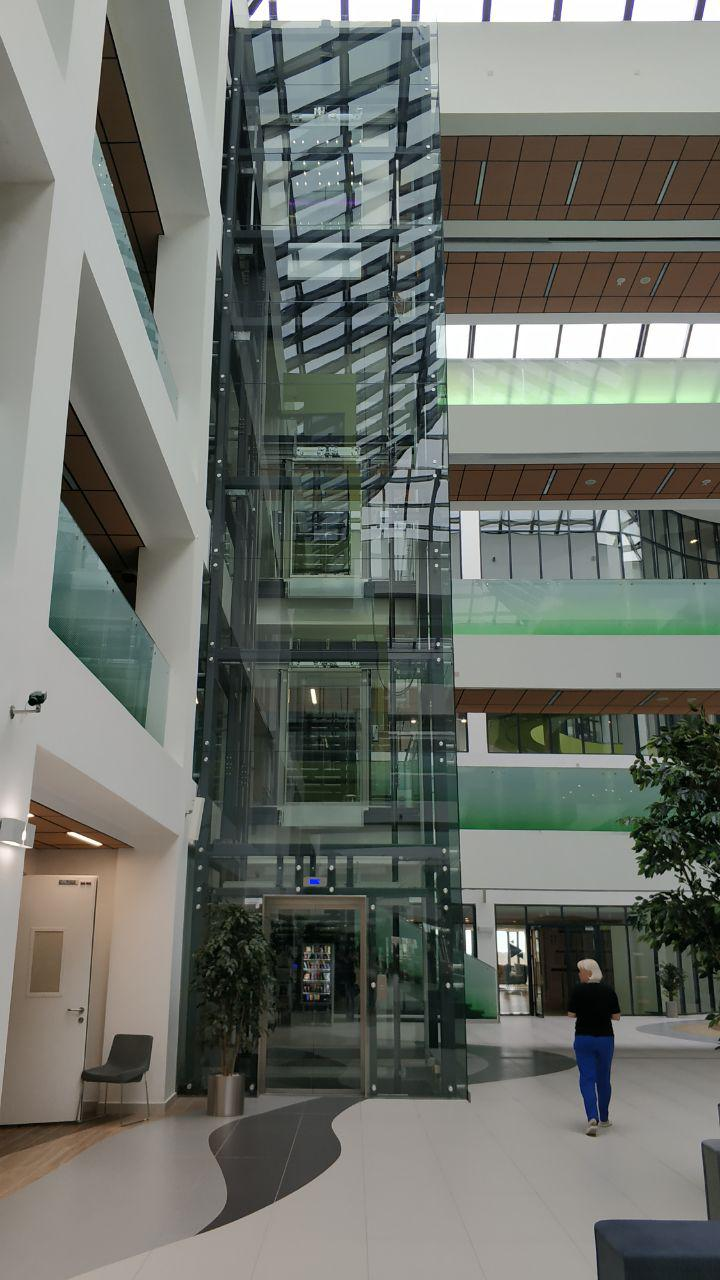
\includegraphics[width=5cm]{history/info/fintex/i3}
    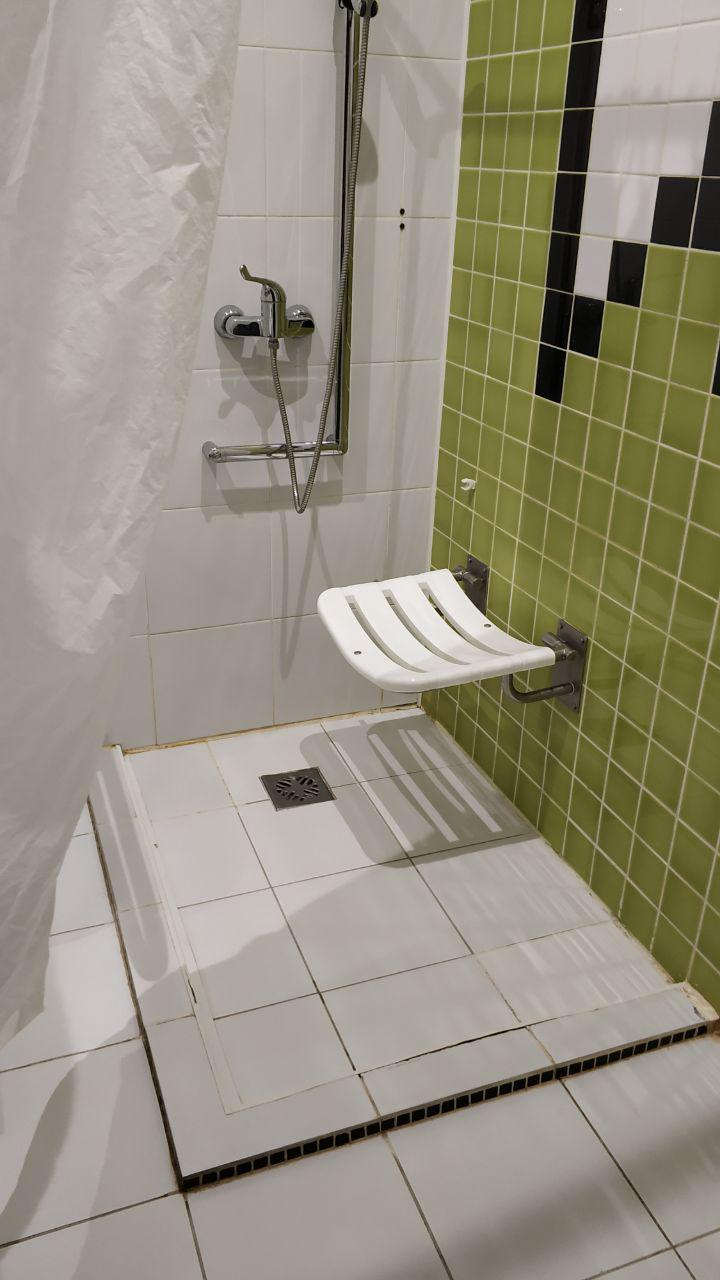
\includegraphics[width=5cm]{history/info/fintex/i4}
\end{center}
\end{figure}

Большинство площадок проведения финалов олимпиады оснащены паспортами доступности для инвалидов объектов и предоставляемых в этих объектах услуг.

При проведении олимпиады в случае необходимости возможно сопровождение детей с ОВЗ ассистентами (сопровождающие лица или родители), оказывающими участникам с ОВЗ, детям-инвалидам и инвалидам необходимую техническую помощь с учетом их индивидуальных особенностей, помогающими им занять рабочее место, передвигаться, прочитать задания. 

В заключительных этапах олимпиады 2018/2019 учебного года приняло участие 9 школьников с ОВЗ, для которых были созданы все необходимые условия для полноценной работы и своевременного оказания необходимой медицинской и иной помощи. Во время проведения олимпиады сопровождающие могли сделать экспресс-анализ крови, дать при необходимости лекарство, сделать укол. На каждой площадке проведения олимпиады находился дежурный врач, который оказывал необходимую медицинскую помощь в т.ч. и детям с ОВЗ.

\section*{Подготовка участников}

Для вовлечения участников в олимпиаду были разработаны «Урок НТИ» и «Демо-этап» олимпиады, благодаря чему участники могли определиться с выбором профилей и попробовать свои силы.

«Урок НТИ» (\url{http://nti-contest.ru/ntilessonteacher/}) – это инициатива Олимпиады НТИ, проходившая в сентябре 2018 года и направленная на распространение информации об НТИ среди школьников и привлечение их к Олимпиаде НТИ через проведение уроков и занятий в школах и учреждениях дополнительного образования. Учебный материал для проведения «Урока НТИ» сформирован в виде конструктора, с помощью которого учителя могли собрать урок по теме НТИ. Урок позволяет познакомить учащихся НТИ и  с профилями Олимпиады НТИ, организовать практическую работу по решению задач в рамках выбранного профиля. Для участия в проекте «Урок НТИ» зарегистрировалось 2185 педагогов.

Демо-этап Олимпиады НТИ (\url{https://stepik.org/course/24389/syllabus}) – это публикация задач олимпиады в открытом доступе. Демо-этап создан для знакомства с задачами по профилям олимпиады, тренировки и испытания собственных знаний и умений решать непростые инженерные задачи.  Прежде чем определиться с участием в олимпиаде и выбором профиля,  потенциальные участники и их наставники могут познакомиться с задачами и выбрать наиболее интересный для себя профиль.

Чтобы участники могли восполнить недостаток практических компетенций и изучить оборудование, на котором им предстоит работать на заключительном этапе Олимпиады НТИ, разработчики направлений представляют методические материалы для самостоятельной практики и самоподготовки, проводят вебинары для участников и педагогов с ответами на вопросы и подбирают подготовительные курсы, совместно с площадками подготовки проводят хакатоны для участников с возможностью попробовать на практике фрагменты финальной задачи. 

Команды разработчиков профилей с целью эффективной подготовки к Олимпиаде НТИ создали видео разборы задач 2 этапа, которые доступны на канале Олимпиады НТИ, \url{https://www.youtube.com/channel/UCZV1CNpOrDNj7tuWuf35lgw/playlists} в 2018 году разработан курс (веб-сайт: \url{https://stepik.org/course/15697/syllabus}) по подготовке школьников к Олимпиаде НТИ на основе контента олимпиады 2017/2018 учебного года. Курс содержит задачи предметных треков 1 и 3 этапа по предметам: математика, физика, информатика, химия и биология и задачи 2 этапа по профилям олимпиады. Курс может использоваться наставниками и самими участниками для подготовки к олимпиаде следующего года. Формат курса максимально приближает участников к реальным условиям олимпиады.

Все указанные материалы находятся в свободном доступе и размещены на официальном сайте олимпиады, на страницах профилей в разделе «Материалы для участников». 

Материалы по профилю «Интеллектуальные робототехнические системы»: \url{http://nti-contest.ru/profiles/irs/}

Олимпиада НТИ является промежуточным итогом работы по реализации дорожной карты НТИ «Кружковое движение»: подготовка к ней велась в фаблабах, ЦМИТах, детских технопарках, на базе активных школ и лицеев, центров дополнительного образования по всей России. Рабочая группа «Кружковое движение» НТИ направлена на развитие технологического сообщества, объединяющего школьников и студентов, ориентированных на инженерную деятельность на рынках НТИ, самодеятельных технических энтузиастов, лидеров технологических кружков, разработчиков педагогических технологий, технологических предпринимателей, популяризаторов науки и технологий.

\section*{Популяризация Олимпиады НТИ}

Олимпиада НТИ широко освещается в различных средствах массовой информации (телевидение, печатные издания, электронные издания). В период с 15 августа 2018 года (начало подготовки к регистрациям) до 3 апреля 2019 года, по данным Медиалогии, Олимпиада НТИ упоминалась в СМИ 2 301 раз, из них 633 раза на федеральном уровне, 1655 на региональном уровне, 13 на зарубежном уровне. 

Во время проведения отборочных этапов Олимпиада НТИ освещалась в федеральных, массовых, родительских, образовательных и иных медиа («ИТАР-ТАСС», «РИА-Новости», «Интерфакс», «Такие Дела», «Летидор», «Дети.Мэйл.ру», «Индикатор», «Занимательная робототехника», «Чердак.Ру», «Habrahabr», «Rusbase», \linebreak «Учёба.Ру»), официальных образовательных порталах и порталах органов государственности власти в регионах  (Новосибирск, Санкт-Петербург, Великий Новгород, Иннополис, Томск, Владивосток, Калининград, Тюмень, Курск, Курган, Тамбов, Мурманск, Новогород, Вологда и т.д.), в печатных изданиях («Российская газета», «Известия»). Радио «Медиаметрикс», программа «Выбор Родителей» под руководством автора самого большого блога для родителей в России.  Кампания по привлечению шла также в научно-популярных группах и группах вузов и площадок партнеров (МАИ, НГУ, Абитуриент НГУ,  ДВФУ, Школьники ДВФУ, Абитуриенты ДВФУ, Мурманский Арктический государственный университет, СибГУ им. М.Ф. Решетнева, Кванториум, АНО ДТ Красноярский кванториум,  НовГУ, ТПУ, абитуриенты ТПУ, МГППУ, Московский Политех, школа Летово, технопарк Академгородка, Сколтех, Иннополис, группы довузовского управления университета Иннополис, Политех Петра, ИТМО, ИРНИТУ, студенты ИРНИТУ, АУ УР РЦИиОКО, Детский технопарк INGENERIKA, Инкубатор Профи, Центр компетенций для детей Поколение 2035, Лаборатория НГУ Инжевика, Чеченский государственный университет, Айти школа Орбита, Фонд Книту, Фонд Золотое сечение, ЦМИТЫ Коптер, Ноосфера, Рекорд, Уникум, Stem-Байкал, Роболатория, Академия Технолаб, Образовательный проект для подростков Tula Teens ,  Проектория, ЯКласс, Фаблаб Политех и другие).  Заключительный этап Олимпиады НТИ в 2018/2019 учебном году проходил при участии журналистов таких печатных изданий, как «Российская газета», «Известия»; федеральных телевизионных каналов («Россия 24» (6 репортажей), «Общественное телевидение России»), федеральных новостных агентств («РИА-Новости», «ИТАР-ТАСС», «Интерфакс») научно-популярных порталов  «Rusbase», «Habrahabr», «Индикатор», «Такие Дела», радиостанций («Радио России», «МедиаМетрикс») Профильные издания освещали соответствующие направления Олимпиады НТИ («Крылья Родины» – «Беспилотные авиационные системы»). В ходе финалов Олимпиады НТИ были инициированы события, вызывающие дополнительный интерес как со стороны участников, так и со стороны СМИ. Так, например в рамках финала в Новосибирском государственном университете, участники встретились с Нобелевским лауреатом Хироси Амано, информация об этом событии была распространена ведущими федеральными агентствами и телеканалами. Разработка победителей профиля «Нейротехнологии», привлекла внимание известной актрисы Екатерины Варнавы, которая написала о своих впечатлениях в блоге с аудиторией 5 млн. 400 тысяч человек, позитивную реакцию на ее пост о победителях олимпиады продемонстрировали больше 75 тысяч пользователей. 

Широкое освещение мероприятий заключительного этапа имеет своей целью распространение информации среди потенциальных участников Олимпиады НТИ будущего года – учеников 7-11 классов и направлено на привлечение талантливых школьников со всей России и активное участие их родителей. В минувшем году была проведена большая работа с целевой аудиторией родителей, чьи дети учатся в 7-11 классах (появилась собственная передача «Выше среднего» на радио Медиаметрикс, регулярно выходят материалы на портале для активных родителей «Летидор», были инициированы эфиры в передача автора самого большого блога для родителей в России (1,6 млн.человек). 

Для привлечения внимания участников к конкретным профилям Олимпиады НТИ ведется точечная работа по освещению их разработок и задач. Инициированы эфиры на радио «Медиаметрикс», тексты в таких медиа как «Rusbase», «Понедельник», «Executive», «БОСС».

В отдельное направление выделена работа с финалистами Олимпиады НТИ с особенными достижениями. Регулярно, а не только в период проведения финалов, инициируются и выходят публикации в таких медиа как: «Российская Газета», «Известия», «Такие Дела», «Индикатор», «RusBase», «Летидор», «Дети Мэйл ру», радио «Медиаметрикс», запущен сервис подкасты в социальной сети ВК, его героями становятся как финалисты, так и разработчики профилей, партнеры, учредители и организаторы Олимпиады НТИ. 
Список лучших материалов об Олимпиаде: \url{http://nti-contest.ru/publications/}.

\chapter{Профиль <<Интеллектуальные робототехнические системы>>}

Профиль ''Интеллектуальные робототехнические системы'', проводимый в
рамках Олимпиады НТИ 2018-2019 учебного года,  был посвящен изучению
алгоритмов компьютерного зрения и межагентрому взаимодейстивию.
Необходимость высокого уровня подготовки участников для решения данных
задач диктовала логику проведения отборочных  этапов: необходимо было
не только выявить школьников, заинтересованных в решении сложной
финальной задачи, но и дать необходимые знания для ее решения.    

Первый отборочный дистанционный этап (индивидуальный) определял общий
уровень подготовки школьников по предметам математика и информатика. 
Решая задачи по программированию, школьники должны были
продемонстрировать простейшие навыки составления и отладки программ,
обрабатывающих  массивы данных, и понимание таких тем, как
комбинаторика, операции со строками, вычислительная геометрия, теория
графов. Задачи по математике проверяли у участников  знания по
алгебре, комбинаторике, геометрии. Количество попыток сдачи решения
задач не ограничивалось. Таким образом, задачи первого этапа выявляли
наличие у участников знаний необходимых не только для решения задач
следующего этапа, но и финальной задачи.

Задачи второго отборочного этапа были разработаны таким образом, что
их было бы сложно решить индивидуальному участнику, поэтому школьники 
должны были объединиться в команды для успешного прохождения в финал. 
Задачи  требовали от участников погружения  в такие робототехнические
темы, как кинематика и навигация робототехнических устройств,
планирование маршрутов перемещения, построение карты с использованием 
экстероцептивных сенсоров, компьютерное зрение, обработка сетевой
информации. Для получения дополнительной информации, необходимой для
решения задач  второго этапа, командам были предложены образовательные
материалы, разработанные в Университете Иннополис.

Команды, прошедшие в финал профиля, приглашались на очный хакатон
(учебно-тренировочные сборы), на котором они могли познакомиться с
аппаратными  особенностями платформы, на которой предстояло решать
задачу финала. В течение сборов команды оттачивали умение управлять
наземным мобильным роботом,  изучали специфику работы с цифровыми
датчиками, реализовывали простейшие алгоритмы обработки изображения,
захваченного с камеры роботототехнического устройства, а также
организовывали передачу информации между несколькими роботами по
беспроводному каналу данных.

Таким образом при решении финальной задачи в очном заключительном
этапе участники могли использовать все знания и наработки, которые они
сделали во  время участия во втором туре и учебно-тренировочных
сборах. Несмотря на то, что задача финала была заранее неизвестна, ее
элементы были рассмотрены на  предварительных этапах, что значительно
упрощало реализацию алгоритма управления робототехническим устройством
в течение 3.5 соревновательных дней.  Дополнительной частью
заключительного этапа являлся индивидуальный тур, в ходе которого
участники решали задачи по математике и информатике.  Задачи по
математике покрывали следующие области математики: оптимизация,
комбинаторика, алгебра и геометрия. А темы задач по информатике
перекликались с классическими темами всероссийской олимпиады
школьников.

\part{Первый этап}
\newpage
\section*{Описание этапа}

Первый отборочный тур проводится индивидуально в сети Интернет,
работы оцениваются автоматически средствами системы
онлайн-тестирования.
Для каждой из параллелей (9 класс или 10-11
класс)
предлагается свой набор задач по математике, задачи по информатике общие
для всех участников. Решение задач по информатике предполагало
написание программ. Участники не были ограничены в выборе языка программирования для
решения задач. На решение
задач каждого предмета первого отборочного этапа участникам давалось 2
дня. У участников было три временных слота по 2 дня каждый, когда они
могли решать задачи по предмету. Решение каждой задачи дает
определенное количество баллов.

Участники получают оценку за решение задач
в совокупности по всем предметам данного профиля (математика и
информатика) --- суммарно от 0 до 200 баллов.

\chapter{Задачи первого этапа. Математика.}

\section{Первая попытка. Задачи 9 класса.}

\subimport{1st_tour/math/try_1/}{math_try_1_9.tex}

\section{Первая попытка. Задачи 10-11 класса.}

\subimport{1st_tour/math/try_1/}{math_try_1_10_11.tex}

\section{Вторая попытка. Задачи 9 класса.}

\subimport{1st_tour/math/try_2/}{math_try_2_9.tex}

\section{Вторая попытка. Задачи 10-11 класса.}

\subimport{1st_tour/math/try_2/}{math_try_2_10_11.tex}

\section{Третья попытка. Задачи 9 класса.}

\subimport{1st_tour/math/try_3/}{math_try_3_9.tex}

\section{Третья попытка. Задачи 10-11 класса.}

\subimport{1st_tour/math/try_3/}{math_try_3_10_11.tex}

\chapter{Задачи первого этапа. Углубленная информатика.}

\section{Первая попытка.}

\subimport{1st_tour/inf2/try_1/}{inf2_try_1.tex}

\section{Вторая попытка.}

\subimport{1st_tour/inf2/try_2/}{inf2_try_2.tex}

\section{Третья попытка.}

\subimport{1st_tour/inf2/try_3/}{inf2_try_3.tex}

\part{Второй этап}
\newpage
\section*{Описание этапа}

Второй отборочный этап проводится в командном формате в сети
интернет, работы оцениваются автоматически средствами системы
онлайн-тестирования.
Продолжительность второго этапа составляет 52 дня. Задачи
по информатике носят междисциплинарный характер и помогают отработать те
навыки, которые потребуются для решения командной задачи заключительного этапа.

Участники не были ограничены в выборе языка программирования для решения задач.

Объем и сложность задач этого этапа подобраны таким образом,
чтобы решение всех задач одним человеком было маловероятно. Это
призвано обеспечить включение командной работы и распределения
обязанностей. Решение каждой задачи дает определенное количество
баллов. Баллы зачисляются в полном объеме за
правильное решение задачи.
Также существуют задачи, где допускается частичное решение.
В данном этапе можно получить суммарно от
0 до 138 баллов.

Задачи по программированию выкладывались
тремя партиями: в начале второго этапа, через три недели после начала
и через шесть недель после начала.
Команды могут выполнять задачи в любом порядке. Задачи допускают
неограниченное число попыток сдать решение.

\chapter{Задачи второго этапа}
\section{Задачи}

\assignementTitle{Запуск всенаправленной тележки}{5}

Робот, моторы которого расположены под углом в $120^{\circ}$ друг к другу,
движется в некотором направлении, пока на моторы подается мощность.
Каждый мотор работает некоторое время: $t_1$,~$t_2$,~$t_3$, соответственно.
На валах моторов закреплены омниколёса (\url{https://en.wikipedia.org/wiki/Omni_wheel}).
С некоторой кинематической моделью робота можно познакомиться по ссылке:
\url{https://bharat-robotics.github.io/blog/kinematic-analysis-of-holonomic-robot/}.

Необходимо определить новые координаты центра робота, если в момент начала движения он находился в точке
$(0,0)$ и один из двигателей находился на оси $Y$, в направлении положительной части (см. рис. \ref{fig:sampleOnceStarted}).
Расположение моторов является постоянным и соответствует рисунку \ref{fig:sampleOnceStarted}.

Считать, что мощность на все моторы подаётся одновременно и достигается мгновенно.
Также считать что происходит движение без поворотов,
иначе говоря робот двигается только прямолинейно в любом направлении.
Колёса вращаются без проскальзывания.

Данные в тестах подобраны таким образом, что нет вариата движения, когда робот движется вокруг какой-то точки.


\putImgForRef{8cm}{2nd_tour/irs/01_Tribot/tribot_configuration}
{Расположение моторов робота относительно центра глобальной системы отсчета в начальный момент времени}{fig:sampleOnceStarted}


\inputfmtSection

Одна строчка, состоящая из 7ми чисел: $d,$~$w_1,$~$t_1,$~$w_2,$~$t_2,$~$w_3,$~$t_3$, разделёнными пробелами, где
\begin{itemize}
    \item $d$ --- диаметр колёс в мм ($30 \leq d \leq 100$);
    \item $w_1, w_2, w_3$ --- скорости вращения моторов в рад/с ($-2$ $\leq w_1, w_2, w_3 \leq 2$);
    \item $t_1, t_2, t_3$ --- время работы каждого мотора в с ($10 \leq t_1, t_2, t_3 \leq 1000$).
\end{itemize}

Диаметр колёс и время движения --- целые числа, скорости вращения --- вещественные.

\commentsSection

Дополнительные наборы входных данных доступны по \url{http://bit.ly/2RdizA3}{ссылке}.

\outputfmtSection


Одна строка, содержащая два целых числа  через пробел  --- координаты центра робота в мм,
где он закончил своё движение.
Допускается погрешность в 1 мм по каждой из координат.

\exampleSection

\sampleTitle{1}


\begin{myverbbox}[\small]{\vinput}
    35 1 15 0 0 -1 15
\end{myverbbox}
\begin{myverbbox}[\small]{\voutput}
    196.875 -113.666
\end{myverbbox}
\inputoutputTable

\sampleTitle{2}

\begin{myverbbox}[\small]{\vinput}
    40 1.4 100 -1.4 100 1.4 100
\end{myverbbox}
\begin{myverbbox}[\small]{\voutput}
    2800 2424.87
\end{myverbbox}
\inputoutputTable


\includeSolutionIfExistsByPath{2nd_tour_progr/01_Tribot/01_move_once_started/solution}
\assignementTitle{Управление всенаправленной тележкой}{10}

Робот, моторы которого расположены под углом в $120^{\circ}$ друг к другу,
движется в заданном направлении некоторое время $t$.
На валах моторов закреплены омниколёса (\url{https://en.wikipedia.org/wiki/Omni_wheel}).
С некоторой кинематической моделью робота можно познакомиться по ссылке:
\url{https://bharat-robotics.github.io/blog/kinematic-analysis-of-holonomic-robot/}.


Необходимо определить новые координаты центра робота,  если в момент начала движения он находился в точке
$(0,0)$ и один из двигателей находился на оси $Y$, в направлении положительной части (см. рис. \ref{fig:sampleMulSstarted}).
Расположение моторов является постоянным и соответствует рисунку \ref{fig:sampleMulSstarted}.

\putImgForRef{8cm}{2nd_tour/irs/01_Tribot/tribot_configuration}
{Расположение моторов робота относительно центра глобальной системы отсчета в начальный момент времени}{fig:sampleMulSstarted}

Считать, что мощность достигается мгновенно и может подаваться на все моторы одновременно.
Колёса вращаются без проскальзывания.
В случае когда на моторы ничего не подаётся, их скорость равна $0$.


\inputfmtSection
Первая строчка содержит четыре целых числа через пробел -- $d,$~$p,$~$t,$~$N$, где:

\begin{itemize}
    \item $d$ --- диаметр колёс в мм ($30 \leq d \leq 100$);
    \item $p$ --- длина оси~(осевой балки) от центра робота до колеса в мм ($ 50 \leq p \leq 125$);
    \item $t$ --- общее время работы моторов в с ($10 \leq t \leq 1000$);
    \item $N$ --- количество измерений ($1 \leq N \leq 1000$).
\end{itemize}


Далее идут $3$ строки --- для первого, второго и третьего моторов, соотвественно.

В каждой строке находится $N$ вещественных чисел через пробел ---  подаваемая на мотор скорость $w_i$, через равные промежутки
времени. ($-2$ рад/с $\leq w_i \leq 2$ рад/с)


\outputfmtSection

Одна строка, содержащая два целых числа  через пробел  --- координаты центра робота в мм,
где он закончил своё движение.
Допускается погрешность в 1 мм по каждой из координат.


\exampleSection

\sampleTitle{1}


\begin{myverbbox}[\small]{\vinput}
    30 50 12 4
    0 0 2 2
    -2 -2 0 0
    2 2 2 2
\end{myverbbox}
\begin{myverbbox}[\small]{\voutput}
    77.486 167.373
\end{myverbbox}
\inputoutputTable

\sampleTitle{2}

\begin{myverbbox}[\small]{\vinput}
    35 55 16 8
    -0.8 -0.8 -0.8 0.6 0.6 0.6 0 0
    -0.8 -0.8 -0.8 0 0 0 0 0
    0.8 0.8 0.8 0.6 0.6 0.6 0 0
\end{myverbbox}
\begin{myverbbox}[\small]{\voutput}
    1.504 130.544
\end{myverbbox}
\inputoutputTable


\includeSolutionIfExistsByPath{2nd_tour/irs/01_Tribot/02_move_multiple_starting/solution}

\assignementTitle{Определение размера препятствия}{15}

Робот, собранный по дифференциальной схеме, передвигается по полигону.
Он оснащён приёмником и дальномером.
Приёмник позволяет измерять расстояния до установленных на поле и находящихся в прямой видимости маяков.
Дальномер направлен влево по ходу движения робота и позволяет получать информацию
о находящихся препятствиях в данном направлении.
На полигоне находятся препятствие и $K$ маяков, координаты которых передаются через входной файл.
Гарантируется, что маяки не мешают роботу перемещаться и не попадают в поле зрения дальномера.
Пример полигона представлен на рис. \ref{fig:beaconFieldExample}.

Необходимо найти площадь препятствия, расположенного на полигоне.
Известно что, приёмник возвращает значения расстояний до препятствия в мм, считая от оси вращения робота,
находящейся в центре между колёсами. Дальномер расположен в том же месте, что и приёмник.

\putImgForRef{8cm}{2nd_tour_progr/02_Beacons/01_beacon_searching/beacons}
{Пример соревновательного полигона}{fig:beaconFieldExample}

\inputfmtSection

Первая строка содержит 3 целых числа: $K$ и $N$ и $dT$:
\begin{itemize}
    \item $K$ --- количество маяков ($10 \leq K \leq 100$);
    \item $N$ --- количество замеров ($10 \leq N \leq 10~000$);
    \item $dT$ --- пауза между измерениями в мс ($0 \leq dT \leq 10~000$).
\end{itemize}

Далее идёт $K$ строк. Каждая строка имеет следующую структуру:
$i$,~ $x_i$,~ $y_i$, в которой все числа вещественные и разделены пробелами, где:
\begin{itemize}
    \item $i$ --- номер маяка по порядку ($0 \leq i \leq 10~000$);
    \item $x_i$ --- координата $x$ $i$-того маяка ($-10~000 \leq x_i \leq 10~000$);
    \item $y_i$ --- координата $y$ $i$-того маяка ($-10~000 \leq y_i \leq 10~000$).
\end{itemize}

Далее идёт $N$ строк. Каждая строка содержит:
\begin{itemize}
    \item $d$ --- целое число, показание дальномера в мм ($0 \leq d \leq 1~000$), в случае если предмет
    находится вне поля видимости дальномера, то его значение будет равно $1~000$;
    \item $Value_{1} ~Value_2 ~\dots ~Value_k$ --- вещественные числа, показания, получаемые приёмником с каждого маяка.
    В случае, если маяк находится вне зоны видимости, то соответствующее значение будет равно $-1$.
\end{itemize}

Все числа указаны через пробел.

\outputfmtSection

Одна строка, содержащая одно целове число -- площадь препятствия в мм$^2$.
Допускается погрешность в $\pm 1$ м$^2$.

\exampleSection

Примеры входных данных и ответов к ним можно найти по \href{http://bit.ly/2Re5l9N}{данной} сслыке.




\includeSolutionIfExistsByPath{2nd_tour_progr/02_Beacons/01_beacon_searching/solution}
\assignementTitle{Определение цветных цилиндров}{15}


Робот, собранный по дифференциальный схеме и оснащенный дальномером, направленным прямо по ходу движения,
перемещается по робототехническому полигону.
На данном полигоне установлены цилиндры различного цвета. Робот также является цилиндром.

В процессе своего передвижения по полигону (см рис. \ref{fig:colourCylindersExample})
робототехническое устройство измерило расстояние до возникающих прямо препятствий
и их цвет в шестнадцатиричном формате вида $RRGGBB$, где $RR$ - 16тиричное число $R$ составляющей данного элемента
матрицы, $GG$ и $BB$ - 16тиричные числа $G$ и $B$ составляющих, соответственно.

\putImgForRef{8cm}{2nd_tour/irs/02_Beacons/02_colour_cylinders/beacons2}
{Пример соревновательного полигона}{fig:colourCylindersExample}

Необходимо определить между какими цилиндрами робот не сможет проехать, если известен маршрут робота и показания
датчика в процессе движения.
Размер цилиндров и робота: $20$ см в диаметре.
Дальномер возвращает расстояние до цилиндра, считая от оси вращения робота,
находящейся в центре между колёсами.
Также гарантируется, что робот измерил каждый цилиндр не менее трех раз, и разница между этими измерениями составляет
минимум $5$ дуговых градусов (при измерении по дуге цилиндра).

\inputfmtSection

Первая строка содержит 2 целых числа: $N$ и $dT$:
\begin{itemize}
    \item $N$ --- количество замеров ($10 \leq N \leq 10000$);
    \item $dT$ --- пауза между измерениями в мс ($0 \leq dT \leq 10000$).
\end{itemize}

Далее идёт $N$ строк. Каждая строка имеет следующую структуру:
$Vel_{linear}$, $Vel_{angular}$, $Distance$, $Color$, в которой все числа разделены пробелами, где:
\begin{itemize}
    \item $Vel_{linear}$ --- линейная скорость в см/с, с которой движется робот в данный момент ($-100 \leq Vel_{linear} \leq 100$);
    \item $Vel_{angular}$ --- угловая скорость в рад/мс, с которой движется робот в данный момент ($-10 \leq Vel_{angular} \leq 10$);
    \item $Distance$ --- показания датчика расстояния в см в диапазоне ``5--255'' см, если предмет вне зоны видимости, то
    будет выведено $255$;
    \item $Color$ --- цвет обнаруженного циллиндра в шестнадцатиричном формате вида $RRGGBB$.
    В случае если цилиндр не обнаружен, будет выведено ``000000''.
\end{itemize}

Значения скоростей и показания датчика являются вещественными числами. Моторы достигают скоростей мгновенно. Робот движется без проскальзывания.
Значения цвета --- целые числа.


\outputfmtSection

Одна строка, в которой указана пара цветов цилиндров в шестнадцатиричной записи через пробел, в порядке возрастания чисел.
В случае если таких пар несколько, то каждую пару следует выводить в отдельной строке.
Несколько строк следует выводить в порядке возрастания первых чисел, а в случае их равенства, в порядке возрастания вторых.


\exampleSection

Примеры входных данных и ответов к ним можно найти по сслыке \url{http://bit.ly/2UoC22Z}.



\includeSolutionIfExistsByPath{2nd_tour/irs/02_Beacons/02_colour_cylinders/solution}

\assignementTitle{Определения расстояния до препятствия}{5}

Камера статично установлена на высоте $h$ мм и отклонена на $\alpha^\circ$ от горизонта.
Она имеет разрешение $height\times width$ и угол обзора $\beta^\circ$.
Поясняющая картинка представлена на рисунке \ref{fig:cameraExample}.

\putImgForRef{8cm}{2nd_tour/irs/03_Camera/01_get_distance/camera_example}
{Схема установки камеры}{fig:cameraExample}


Необходимо найти расстояние до предмета, установленного на полигоне.
Гарантируется, что предмет находится в поле зрения камеры, является однотонным.
Его минимальная площадь на изображении равна $s \%$.
Также известно, что помимо требуемого предмета
в камеру попадает поверхность полигона и(или) борта.
Поверхность полигона не однородная, а содержащая различные цвета в хаотическом порядке.

Пример изображения представлен на рис.  \ref{fig:getDistanceImageExample},

\putImgForRef{8cm}{2nd_tour/irs/03_Camera/01_get_distance/field_example}
{Пример изображения с камеры}{fig:getDistanceImageExample}


\inputfmtSection

Первая строка входного файла содержит 6 чисел: $h$,~ $\alpha$,~ $\beta$,~ $height$,~ $width$,~$s$:
\begin{itemize}
    \item $h$ --- высота установки камеры в мм ($10 \leq h \leq 100$);
    \item $\alpha$ --- угол в градусах,  под которым расположена камера относительно горизонта ($0^\circ \leq \alpha \leq 45^\circ$);
    \item $\beta$ --- угол обзора камеры в градусах ($30^\circ \leq \alpha \leq 180^\circ$);
    \item $height$ --- разрешение изображения по высоте ($10 \leq height \leq 2000$);
    \item $width$ --- разрешение изображения по ширине ($10 \leq width \leq 2000$);
    \item $s$ --- минимальная площадь предмета в $\%$ от всего изображения, которое измеряется в пикселях ($1 \leq s \leq 100$).
\end{itemize}

На следующих $height$ строках расположено изображение размером $height\times width$ в виде шестнадцатиричных чисел.
Данные числа имеют следующий вид: $RRGGBB$, где $RR$ - 16тиричное число $R$ составляющей данного элемента
матрицы, $GG$ и $BB$ - 16тиричные числа $G$ и $B$ составляющих, соответственно.

Все числа являются целыми.


\outputfmtSection

Одна строка, в которой указано число --- расстояние до предмета в мм. Допускается погрешность в 10 мм.


\exampleSection

Примеры входных данных и ответов к ним можно найти по сслыке \url{http://bit.ly/2FCbgAU}.


\includeSolutionIfExistsByPath{2nd_tour/irs/03_Camera/01_get_distance/solution}
\assignementTitle{Определение вектора перемещения робота в заданном виде}{20}


Робот, собранный по дифференциальной схеме, оборудован камерой.
Камера установлена так, что смотрит вниз перпендикулярно поверхности, по которой движется робот.
Известны характеристики камеры такие, как разрешение ($height\times width$),
угол обзора $\alpha$, высота расположения над плоскостью движения.
Верхний край кадра находится дальше от робота, чем нижний край кадра.

Есть последовательность кадров, сделанных камерой через равные промежутки времени.
Всего кадров было сделано $N$.

\putImg{8cm}{2nd_tour/irs/03_Camera/02_find_velocity/robot_example}
{Вид робота. Поясняющая картинка}


Зная, что робот движется с постоянной линейной $(v)$ и постоянной угловой $(\omega)$ скоростью,
необходимо определить перемещение по $X$ и по $Y$ в мм.

\inputfmtSection

Входной файл состоит из нескольких строк.

Первая строка содержит 5 целых чисел: $N$,~ $h$,~ $\alpha$,~ $height$,~ $width$:
\begin{itemize}
    \item $N$ --- количество замеров камерой ($2 \leq N \leq 16$);
    \item $h$ --- высота установки камеры в мм ($10 \leq h \leq 2000$);
    \item $\alpha$ --- угол обзора камеры в градусах ($15^\circ \leq \alpha \leq 175^\circ$);
    \item $height$ --- разрешение изображения по высоте ($5 \leq height \leq 16$);
    \item $width$ --- разрешение изображения по ширине ($5 \leq width \leq 16$).
\end{itemize}

Далее расположено $N$ строк, на каждой из которых расположено изображение размером
$height\times width$ в виде шестнадцатиричных чисел слева направо, сверху вниз.
Данные числа имеют следующий вид: $RRGGBB$, где $RR$ - 16тиричное число $R$ составляющей данного элемента
матрицы, $GG$ и $BB$ --- 16тиричные числа $G$ и $B$ составляющих соответственно.

Все числа являются целыми.


\outputfmtSection

Вывести пару вещественных чисел с точностью до целых --- перемещение по $X$ и по $Y$  в мм в данном порядке через пробел.


\exampleSection

Примеры входных данных и ответов к ним можно найти по сслыке \url{http://bit.ly/2EP1c5g}.





\includeSolutionIfExistsByPath{2nd_tour/irs/03_Camera/02_find_velocity/solution}
\assignementTitle{Распознавание ARTag маркера}{10}

Для определения своего местоположения квадрокоптер использует камеру, снимающую поверхность,
над которой перемещается робот. Изображение с камеры приходит в управляющую
программу в виде набора $height \times width$ точек, где каждая точка закодирована в RGB-формате.


\putImgForRef{8cm}{2nd_tour/irs/03_Camera/03_ArTag_detecting/arTag_description}
{Нумерация битов в маркера}{fig:arTagDescription}

На поверхность нанесены ARTag маркеры (\url{https://inside.mines.edu/~whoff/courses/EENG512/lectures/other/ARTag.pdf}).
Элементы маркера, расположенные по его границе - всегда черные. Четыре элемента,
находящиеся в углах внутреннего $3\times 3$ квадрата определяют ориентацию маркера таким
образом, что только элемент в нижнем правом углу квадрата - белый. Центральный элемент
квадрата используется для проверки четности (parity check): если количество единичных бит в двоичной
записи закодированного в маркере числа нечетное, то он черный. Оставшиеся $4$ элемента маркера
кодируют число по следующему правилу: если элемент черный, то в он обозначает $1$,
если белый, то $0$ при этом самый первый элемент --- старший бит закодированного числа.
Элементы пронумерованы сверху вниз, слева направо (см. рис. \ref{fig:arTagDescription}).

Например, на маркере с рис. \ref{fig:arTagExample} закодировано число $0011_2$, что
эквивалентно $3_{10}$.

\putImgForRef{8cm}{2nd_tour/irs/03_Camera/03_ArTag_detecting/arTag_example}
{Маркер с закодированным значением - $0011_2$}{fig:arTagExample}

Поскольку квадрокоптер не перемещается постоянно параллельно поверхности, то изображения
ARTag маркера, получаемые с камеры, получаются в виде неправильного выпуклого
четырехугольника, а непостоянные условия освещенности изменяют фокус, тон и добавляют блики на изображение.
Также квадрокоптеру не всегда удается полностью захватить маркер, и необходимо обрабатывать данные с нескольких снимков.


Поскольку направление запуска квадрокоптера заранее неизвестно, то ориентация маркеров
заранее неизвестна, но его изображение таково, что оно по каждой из осей $X, Y, Z$
относительно оптической оси камеры не превышает $25$ градусов.

Напишите программу для определения закодированного в маркере числа.

\inputfmtSection

Входной файл состоит из нескольких строк.

Первая строка содержит 3 целых числа: $N$,~ $height$,~ $width$:
\begin{itemize}
    \item $N$ --- количество замеров камерой ($1 \leq N \leq 100$);
    \item $height$ --- разрешение изображения по высоте ($10 \leq height \leq 1000$);
    \item $width$ --- разрешение изображения по ширине ($10 \leq width \leq 1000$).
\end{itemize}

Далее расположено $N$ строк на каждой расположено изображение размером
$height\times width$ ввиде шестнадцатиричных чисел слева направо сверху вниз.
Данные числа имеют следующий вид: $RRGGBB$, где $RR$ - 16тиричное число $R$ составляющей данного элемента
матрицы, $GG$ и $BB$ --- эт0 16ти-ричные числа $G$ и $B$ составляющих соответственно.

Все числа являются целыми.

\outputfmtSection
Вывести одно целое число в десятичной системе счисления, которое было закодированное на маркере.
В случае если невозможно определить число, следует вывести $-1$.


\exampleSection


Примеры входных данных и ответов к ним можно найти по сслыке \url{http://bit.ly/2DHww5w}.




\includeSolutionIfExistsByPath{2nd_tour/irs/03_Camera/03_ArTag_detecting/solution}

\assignementTitle{Определение лабиринта}{10}

Роботы в количестве $N$, собранные по дифференциальной схеме, оснащёны тремя дальномерами, направленными налево, прямо и
направо относительно направления движения робота.
Роботы движутся одновременно  из заранее известных секторов по неизвестному лабиринту, размером $K \times M$ секторов.

Между секторами могут быть стены, нахождение препятствия, внутри сектора недопустимо.
Отсчёт координат секторов начинается с $(0;0)$ в левом верхнем углу, $X$  возрастает вправо, $Y$ --вниз.

В процессе своих перемещений они получают значения с дальномеров, позволяющих узнать структуру лабиринта.
В результате полученных данных необходимо понять в какие сектора полигона может попасть первый робот, без
учёта нахождения на поле других роботов. В случае если данное значение невозможно определить,
следует вывести количество секторов, посещённых в процессе движения данным роботом.

\putImg{8cm}{2nd_tour/irs/04_Multiple_agents/01_maze_structure_detecting/field_example}
{Пример соревновательного полигона}

\putImg{5cm}{2nd_tour/irs/04_Multiple_agents/01_maze_structure_detecting/sensors_location}
{Расположение датчиков}


\inputfmtSection

Первая строка содержит 4 целых числа: $N$, $K$, $M$ и $i$:
\begin{itemize}
    \item $N$ --- количество роботов на поле $(2 \leq N \leq 5)$;
    \item $K$ --- ширина (по оси $X$) лабиринта в секторах $(4 \leq K \leq 20)$;
    \item $M$ --- длина (по оси $Y$) лабиринта в секторах $(4 \leq M \leq 20)$;
    \item $i$ --- количество показаний каждого робота.
\end{itemize}

Далее идет $N$  строк, содержащие координаты старта каждого робота, а также направление робота при старте,
т.е. одна строка имеет следующую структуру: $x_s$, $y_s$, $dir$, где:
\begin{itemize}
    \item $x_s$ --- координаты старта данного робота по оси $X$;
    \item $y_s$ --- координаты старта данного робота по оси $Y$;
    \item $dir$ --- направление робота при старте:
    \begin{itemize}
        \item $U$ --- робот направлен вверх;
        \item $L$ --- робот направлен влево;
        \item $D$ --- робот направлен вниз;
        \item $R$ --- робот направлен вправо;
    \end{itemize}
\end{itemize}

Далее идет $N$ блоков по $i$ строк.
На каждой строке находится действие робота и показания всех датчиков после этого действия через пробел:
$Movement, ~ D_l,~ D_f, ~D_r$:
\begin{itemize}
    \item $Movement$ --- выполненное действие робота:
    \begin{itemize}
        \item $F$ --- проезд робота в следующий по ходу движения сектор;
        \item $L$ --- поворот робота в данном секторе налево;
        \item $R$ --- поворот робота в данном секторе направо;
    \end{itemize}
    \item $D_l$ --- показания датчика расстояния, направленного влево:
    \begin{itemize}
        \item $1$ --- присутствует препятствие;
        \item $0$ --- отсутствует препятствие;
    \end{itemize}
    \item $D_f$ --- показания датчика расстояния, направленного вперёд:
    \begin{itemize}
        \item $1$ --- присутствует препятствие;
        \item $0$ --- отсутствует препятствие;
    \end{itemize}
    \item $D_r$ --- показания датчика расстояния, направленного вправо:
    \begin{itemize}
        \item $1$ --- присутствует препятствие;
        \item $0$ --- отсутствует препятствие.
    \end{itemize}
\end{itemize}



\outputfmtSection

Одно число - количество секторов, которое возможно посетить. Если невозможно определить, то вывести число
секторов посещённых первым роботом.


\exampleSection

Примеры входных данных и ответов к ним можно найти по сслыке \url{http://bit.ly/2LK5FrH}.





\includeSolutionIfExistsByPath{2nd_tour/irs/04_Multiple_agents/01_maze_structure_detecting/solution}
\assignementTitle{Планирование движения в лабиринте}{15}

Роботы в количестве $N$, собранные по дифференциальной схеме, движутся по заранее известному лабиринту и
представленному на рис. \ref{fig:mazeStructureExample}.

Необходимо доехать из начального в конечный сектор каждым роботом, если они
движутся одновременно и параллельно и имеют следующие команды:
\begin{itemize}
    \item $F$ --- проезд робота в следующий по ходу движения сектор;
    \item $L$ --- поворот робота в данном секторе налево и проезд в следующий по ходу движения сектор;
    \item $R$ --- поворот робота в данном секторе направо и проезд в следующий по ходу движения сектор.
\end{itemize}
Считать что роботы поворачиваются мгновенно, а после одновременно начинают движение вперёд с 
одинаковой скоростью.Робот является цилиндром и занимает 2/3 площади клетки. Каждое перемещение он начинает и 
заканчивает в центре клетки.

Также гарантируется, что данных команд будет достаточно для выполнения задачи. При движении столкновение не 
допускается и перемещение необходимо осуществлять так, чтобы роботы получили наименьшее число команд. Иначе 
говоря, необходимо, чтобы сумма длин строк, содержащих команды передаваемые на робота в хронологическом порядке, 
без пробелов и запятых, была минимально возможной.

\putImgForRef{8cm}{2nd_tour/irs/04_Multiple_agents/02_maze_movement/field_example}
{Структура лабиринта для решения задачи}{fig:mazeStructureExample}

\inputfmtSection

Первая строка содержит 1 целое число: $N$ --- количество роботов на поле \linebreak $(1 \leq N \leq 3)$.

Далее идет $N$ строк, содержащие координаты старта и финиша каждого робота, а также
направление робота при старте, т.е. одна строка имеет следующую структуру:
$x_s$,~ $y_s$,~$dir$,~ $x_f$,~ $y_f$, где:
\begin{itemize}
    \item $x_s$ --- координаты старта данного робота по оси $X$;
    \item $y_s$ --- координаты старта данного робота по оси $Y$;
    \item $dir$ --- направление робота при старте:
        \begin{itemize}
            \item $U$ -- робот направлен вверх;
            \item $L$ -- робот направлен влево;
            \item $D$ -- робот направлен вниз;
            \item $R$ -- робот направлен вправо;
        \end{itemize}
    \item $x_f$ --- координаты финиша данного робота по оси $X$;
    \item $y_f$ --- координаты финиша данного робота по оси $Y$;
\end{itemize}

Все данные указаны через пробел, числа являются целыми.


\outputfmtSection

$N$ строк, каждая строка содержит команды, передаваемые на данного робота в хронологическом порядке
(самая первая команда расположена в начале строки), без пробелов и запятых.


\commentsSection

Дополнительные наборы входных данных доступны по ссылке \url{http://bit.ly/2KtN4z9}.

\exampleSection

\sampleTitle{1}

\begin{myverbbox}[\small]{\vinput}
    2
    6 7 U 0 2
    7 7 U 1 2
\end{myverbbox}
\begin{myverbbox}[\small]{\voutput}
    FLLRFFFFRFFFF
    FLRFFFLLRFFRL
\end{myverbbox}
\inputoutputTable

\sampleTitle{2}

\begin{myverbbox}[\small]{\vinput}
    2
    0 0 D 2 5
    0 1 R 2 1
\end{myverbbox}
\begin{myverbbox}[\small]{\voutput}
    FFFFFFLFL
    RFFFFFLFFLFFLRFRLFLL
\end{myverbbox}
\inputoutputTable




\includeSolutionIfExistsByPath{2nd_tour/irs/04_Multiple_agents/02_maze_movement/solution}

\assignementTitle{Определение пересекающихся траекторий \\}{10}

Имеется набор байт --- трафик, собранный на концентраторе, во время общения в локальной сети нескольких  устройств,
включая робототехнические устройства.

Известно, что робототехнические устройства общались по протоколу, построенному поверх UDP (\url{https://ru.wikipedia.org/wiki/UDP}) и
реализованному следующим образом: три целых числа -- $t_i$,~ $X_i$, ~$Y_i$ -- каждое из которых занимает $4$ байта,
где $t_i$ --- время, в которое были сняты данные показатели координат, а $X_i$ ~и~ $Y_i$ --- координаты местоположения
робототехнической тележки в данный момент времени.
При записи чисел использовалась нотация BigEndian (\url{https://en.wikipedia.org/wiki/Endianness}).

Необходимо определить IP-адреса (\url{https://ru.wikipedia.org/wiki/IPv4}) \linebreak устройств, чьи траектории пересекались.


Считать, что между изменениями робототехнические тележки перемещались прямо.
Гарантируется, что через данный концентратор проходит лишь необходимый трафик, т.е. отсутствуют пакеты,
не относящиеся к данной задаче.

\inputfmtSection


Первая строка содержит 1 целое число: $N$ --- количество переданых пакетов через концентратор  $(4 \leq N \leq 10^3)$.

Далее идут $N$ строк, каждая из которых содержит один пакет, переданный через концентратор в побитовом формате, который содержит
$t_i$,~ $X_i$, ~$Y_i$, где:
\begin{itemize}
    \item $t_i$ --- время в мс, в которое были сняты данные показатели координат~-- $4$~байта $(0 \leq t_i < 2^{32})$;
    \item $X_i$ --- координаты по оси $X$~ местоположения робототехнической тележки в данный момент времени --- $4$ байтa $(0 \leq X_i < 2^{32})$;
    \item $Y_i$ --- координаты по оси $Y$~ местоположения робототехнической тележки в данный момент времени --- $4$ байтa $(0 \leq Y_i < 2^{32})$.
\end{itemize}

\outputfmtSection

Необходимо вывести два IP-адресса в десятичном формате через пробел в порядке их возрастания -- адреса устройств,
чьи траектории пересекались.

В случае если пересекались несколько пар роботов, эти пары следуют в порядке первых пересечений траекторий
робототехнических устройств.

В случае если таких пересечений нет, следует вывести $-1$.

\exampleSection

Примеры входных данных и ответов к ним можно найти по сслыке \url{http://bit.ly/2QkcNzv}.


\includeSolutionIfExistsByPath{2nd_tour_progr/05_Communication/01_Found_intersects/solution}

\assignementTitle{Определение собственных координат}{10}

Робот собранный по дифференциальной схеме оснащен двумя инфракрасными датчиками расстояния. Один из датчиков расстояния установлен так, что показывает расстояние до препятствий прямо по курсу робота. Второй датчик расстояния направлен влево.

\putImgForRef{8cm}{2nd_tour/irs/06_in_simulatior/04_discrete_odometry/maze-002}
{Пример начального расположения робота}{fig:discreteOdometryStartPos}

Для решения задачи робот запускается на поле, состоящим из 8х8 квадратных секторов. На поле между некоторыми секторами установлены препятствия для ограничения перемещения робота.

Роботу необходимо проехать некоторое количество секторов, заданное через входной файл \textit{input.txt}, по правилу ''левой руки'', после остановиться и вывести на экран относительные координаты, т.е. свои координаты относительно точки старта, в формате $(X, Y)$, где начало отсчета - точка старта, направление оси $Y$ совпадает с первоначальным направлением движения, ось $X$ направлена вправо перпендикулярно оси $Y$.

\begin{center}
\noindent
\textbf{Конфигурация робота}
\end{center}

\twoitems{Подключение моторов}{Левый мотор - порт M3;}{Правый мотор - порт M4.}
\twoitems{Подключение датчиков}{Датчик расстояния, направленный вперед - порт A1}
{Датчик расстояния, направленный влево - порт A2}

\inputfmtSection

Входной файл содержит только одну строчку. В строке - целое число $N$ \linebreak $(5 \leq N \leq 40)$, определяющее количество секторов, которое необходимо проехать. Сектор старта не учитывается в подсчёте.

\begin{center}
\noindent
\textbf{Ограничения}
\end{center}

Робот не должен выполнять задание дольше 3 минут.

\exampleSection

Для лабиринта, представленного на рис. \ref{fig:discreteOdometryStartPos}, и при числе $7$ во входных данных, робот должен остановиться в соответствии с рис. \ref{fig:discreteOdometryFinishPos} и вывести на экран $(4,1)$.

\putImgForRef{8cm}{2nd_tour/irs/06_in_simulatior/04_discrete_odometry/maze-002-finish}
{Расположение робота, стартовавшего из позиции на рис. \ref{fig:discreteOdometryStartPos} и проехавшего $7$ секторов}{fig:discreteOdometryFinishPos}

\includeSolutionIfExistsByPath{2nd_tour/irs/06_in_simulatior/04_discrete_odometry/solution}

\part{Заключительный этап}

\clearpage
\chapter{Предметный тур}

На индивидуальное решение задач дается по 2 часа на один предмет.
Для каждой из параллелей (9 класс или 10-11 класс) предлагается свой
набор задач по математике, задачи по информатике - общие для всех
участников.

Решение каждой задачи по математике дает определенное количество
баллов (см. критерии оценки). При этом некоторые задачи делятся на
подзадачи. За каждую подзадачу можно получить от 0 до указанного
количества баллов.

Решение задач по информатике предполагало написание программ.
Ограничения по используемым языкам программирования не было.
Проверочные тесты для каждой задачи по информатике делились на
несколько групп. Прохождение всех тестов в группе тестов дает
определенное количество баллов за решение задачи.

Участники получают оценку за решение задач в совокупности по
всем предметам данного профиля (математика и информатика) ---
суммарно от 0 до 200 баллов.

\begin{itemize}
    \item {\bf Математика 9 класс} количество набранных баллов
    (от 0 до 100);
    \item {\bf Математика 10-11 класс} количество набранных баллов
    (от 0 до 100);
    \item {\bf Информатика} количество набранных баллов (от 0 до
    300) делится на коэффициент 3.
\end{itemize}

\section{Математика. 9 класс}

\subimport{final/subject_tour/math0903_irs_9/task_01/}{statement}
\subimport{final/subject_tour/math0903_irs_9/task_01/}{solution}

\subimport{final/subject_tour/math0903_irs_9/task_02/}{statement}
\subimport{final/subject_tour/math0903_irs_9/task_02/}{solution}

\subimport{final/subject_tour/math0903_irs_9/task_03/}{statement}
\subimport{final/subject_tour/math0903_irs_9/task_03/}{solution}


\section{Математика. 10-11 класс}

\subimport{final/subject_tour/math0903_irs_10/task_01/}{statement}
\subimport{final/subject_tour/math0903_irs_10/task_01/}{solution}

\subimport{final/subject_tour/math0903_irs_10/task_02/}{statement}
\subimport{final/subject_tour/math0903_irs_10/task_02/}{solution}

\subimport{final/subject_tour/math0903_irs_10/task_03/}{statement}
\subimport{final/subject_tour/math0903_irs_10/task_03/}{solution}


\section{Информатика}

\subimport{final/subject_tour/inf0903_irs/task_01/}{statement.tex}
\subimport{final/subject_tour/inf0903_irs/task_02/}{statement.tex}
\subimport{final/subject_tour/inf0903_irs/task_03/}{statement.tex}


\chapter{Командный тур}

В командной части заключительного этапа участники должны
спроектировать автономную систему управления групой роботов-погрузчиков
для решения задач навигации на модели логистического центра с
использованием алгоритмов компьютерного зрения.

Командная часть заключительного этапа проходит в течении
3.5 дней (всего 26 астрономических часов), которые включают работу по
оснащению роботов необходимыми датчиками, программированию, пробные заезды
на макете логистического центра, зачетные попытки.

\subimport{final/command_tour/irs/}{content.tex}

\part{Критерии}

\chapter{Критерии определения победителей и призеров заключительного этапа}
 
\section{Первый отборочный этап}
 
В первом отборочном этапе участники решали задачи по двум предметам - математика и информатика, в каждом предмете максимально можно было набрать 100 баллов. Для того, чтобы пройти во второй этап участники должны были набрать в сумме по обоим предметам:
\begin{itemize}
    \item 9 классы и младше - не менее 80 баллов.
    \item 10-11 класс - не менее 100 баллов.
\end{itemize}

\section{Второй отборочный этап}

Количество баллов, набранных при решении всех задач, суммируется. Призерам второго отборочного этапа было необходимо набрать не менее 40 баллов.

Победители второго отборочного этапа являются финалистами олимпиады и должны были набрать 46 баллов и выше независимо от уровня.

\section{Заключительный этап}

В заключительном этапе олимпиады баллы участника складываются из двух частей: 
\begin{enumerate}
    \item[1 -] участник получает баллы за индивидуальное решение задач по предметам (математика и информатика)
    \item[2 -] участник получает баллы за командное решение практической задачи.
\end{enumerate} 

Итоговый личный балл участника рассчитывается по формуле:
$$S = Si + Sm + St, \: \text{где:}$$
 
$Si$ - сумма баллов по информатике, набранная в рамках индивидуальной части заключительного этапа (максимум 300 баллов), нормированная на 100;

$Sm$ - сумма баллов по математике, набранная в рамках индивидуальной части заключительного этапа (максимум 100 баллов); 

$St$ - количество баллов, набранное в рамках командной части заключительного этапа (максимум 400 баллов).

Критерий определения победителей и призеров:
\begin{center}
    \begin{tabular}{|l|l|}
        \hline
        Категория&Количество баллов\\
        \hline
        Победители&160 баллов и выше\\
        \hline
        Призеры&От 140 до 159 баллов\\
        \hline
    \end{tabular}
\end{center}

\end{document}